\begin{figure}[t!]
\tikzset{%
process/.style  = {rectangle, minimum width=1cm, minimum height=1cm, align=flush center, draw=black, inner sep=0.2cm},
decision/.style = {diamond, minimum width=1cm, minimum height=1cm, align=flush center, draw=black, inner sep=0cm},
resource/.style = {shape=rounded rectangle, minimum width=1cm, minimum height=1cm, align=flush center, draw=black},
stop/.style     = {rectangle, minimum width=1cm, minimum height=1cm, align=flush center, draw=black, double, thick},
waypoint/.style = {coordinate}
}
\newcommand{\cbox}[2]{\parbox{#1}{\centering
#2}}
\newcommand{\mrule}[1]{\rule[0.8ex]{#1}{0.4pt}}
\resizebox{0.5\textwidth}{!}{%
\begin{tikzpicture}[
thick,
>/.tip=Latex,
loose/.style={inner sep 0.7em}]
\draw
	node at (0,0) [font=\large] (statement) {If $\langle \state \rangle$ then $\langle \action \rangle$ because $\langle \goal \rangle$}
	
	node [process, below of=statement, node distance=1.5cm] (parse) {\cbox{3.5cm}{Parse Statement:\\
	$\begin{array}{ccc} \state &\action &\goal \end{array}$}}
	
    node [decision,below of=parse,node distance=3.5cm] (in_k) {\cbox{1.5cm}{Is $\goal$ in \KB?}}
    
    node [decision,right of=in_k,node distance=2.5cm,minimum width=1.5cm] (loop) {$i>n$?}
    
    node [process,right of=loop,node distance=3.5cm] (startFeedback) {\parbox{3.5cm}{Ask the user for more\\ information. \\\mrule{3.5cm} \\ $i=i+1$ \\ $\mathrm{goalStack}.push(\goal)$ \\ $ \goal = G' (Z)$}}
    
        node[waypoint,right of=startFeedback,node distance=2.7cm] (loop_0) {}
        node[waypoint,above of=loop_0,node distance=2cm] (loop_1) {}
        node[waypoint,left of=loop_1,node distance=8.7cm] (loop_2) {}
    
    node[stop,below of=loop,node distance=1.75cm] (fail0) {Fail}
    
    %%
    node[decision,below of=in_k,node distance=4.5cm,minimum width=3cm] (empty) {\cbox{1.5cm}{goalStack empty?}}
    
    node[process,right of=empty,node distance=5cm] (add) {\parbox{4cm}{Add a new rule to K \\ \mrule{3cm} \\ $\mathrm{goalStack}.top() \vdash \goal$ \\ $\goal = \mathrm{goalStack}.pop()$}}
    
        node[waypoint,right of=add,node distance=3cm] (empty_0) {}
        node[waypoint,above of=empty_0,node distance=1.6cm] (empty_1) {}
        node[waypoint,left of=empty_1,node distance=8cm] (empty_2) {}
    
    node[decision,below of=empty,node distance=3.5cm,minimum width=3.5cm] (prove) {\cbox{1.5cm}{Is there a proof for $\goal$?}}
    
    node[resource,above of=prove,node distance=1.5cm,right=1cm] (embeddings0) {\cbox{3cm}{\textcolor{black}{Rule and Variable embeddings}}}
    
    node[stop,right of=prove,node distance=4cm] (fail1) {Fail}

    node[decision,below of=prove,node distance=3.5cm,minimum width=5cm,inner sep=-0.2cm] (check_proof) {\cbox{2.2cm}{Does the \\
    proof contain \\
    $\state$ and $\action$? }}
    
    node[stop,right of=check_proof,node distance=4cm] (fail2) {Fail}
    
    node[stop,below of=check_proof,node distance=3cm] (success) {Succeed};
    
\draw(statement) edge [->] (parse);
\draw(parse) edge [->] (in_k);
%%
\draw(in_k) edge ["Y"',pos=0.05,->] (empty);
\draw(in_k) edge ["N",very near start,->] (loop);
%%
\draw(loop) edge ["Y"',->] (fail0);
\draw(loop) edge ["N",very near start,->] (startFeedback);

    \draw(startFeedback) edge (loop_0);
    \draw(loop_0) edge (loop_1);
    \draw(loop_1) edge ["\textcolor{brickred}{user feedback loop}", ->] (loop_2);
%%
\draw(empty) edge ["Y"',->] (prove);
\draw(empty) edge ["N",near start,->] (add);

    \draw(add) edge (empty_0);
    \draw(empty_0) edge (empty_1);
    \draw(empty_1) edge ["\textcolor{brickred}{updating the knowledge base}",->] (empty_2);
%%
\draw(prove) edge ["Y"',->] (check_proof);
\draw(prove) edge ["N",very near start,->] (fail1);
\draw(prove) edge [dotted] (embeddings0);
%%
\draw(check_proof) edge ["Y"',"\textcolor{brickred}{returns proof, i.e. chain of reasoning}",->] (success);
\draw(check_proof) edge ["N",near start,->]  (fail2);
%%
\end{tikzpicture}
    }%
    
    % 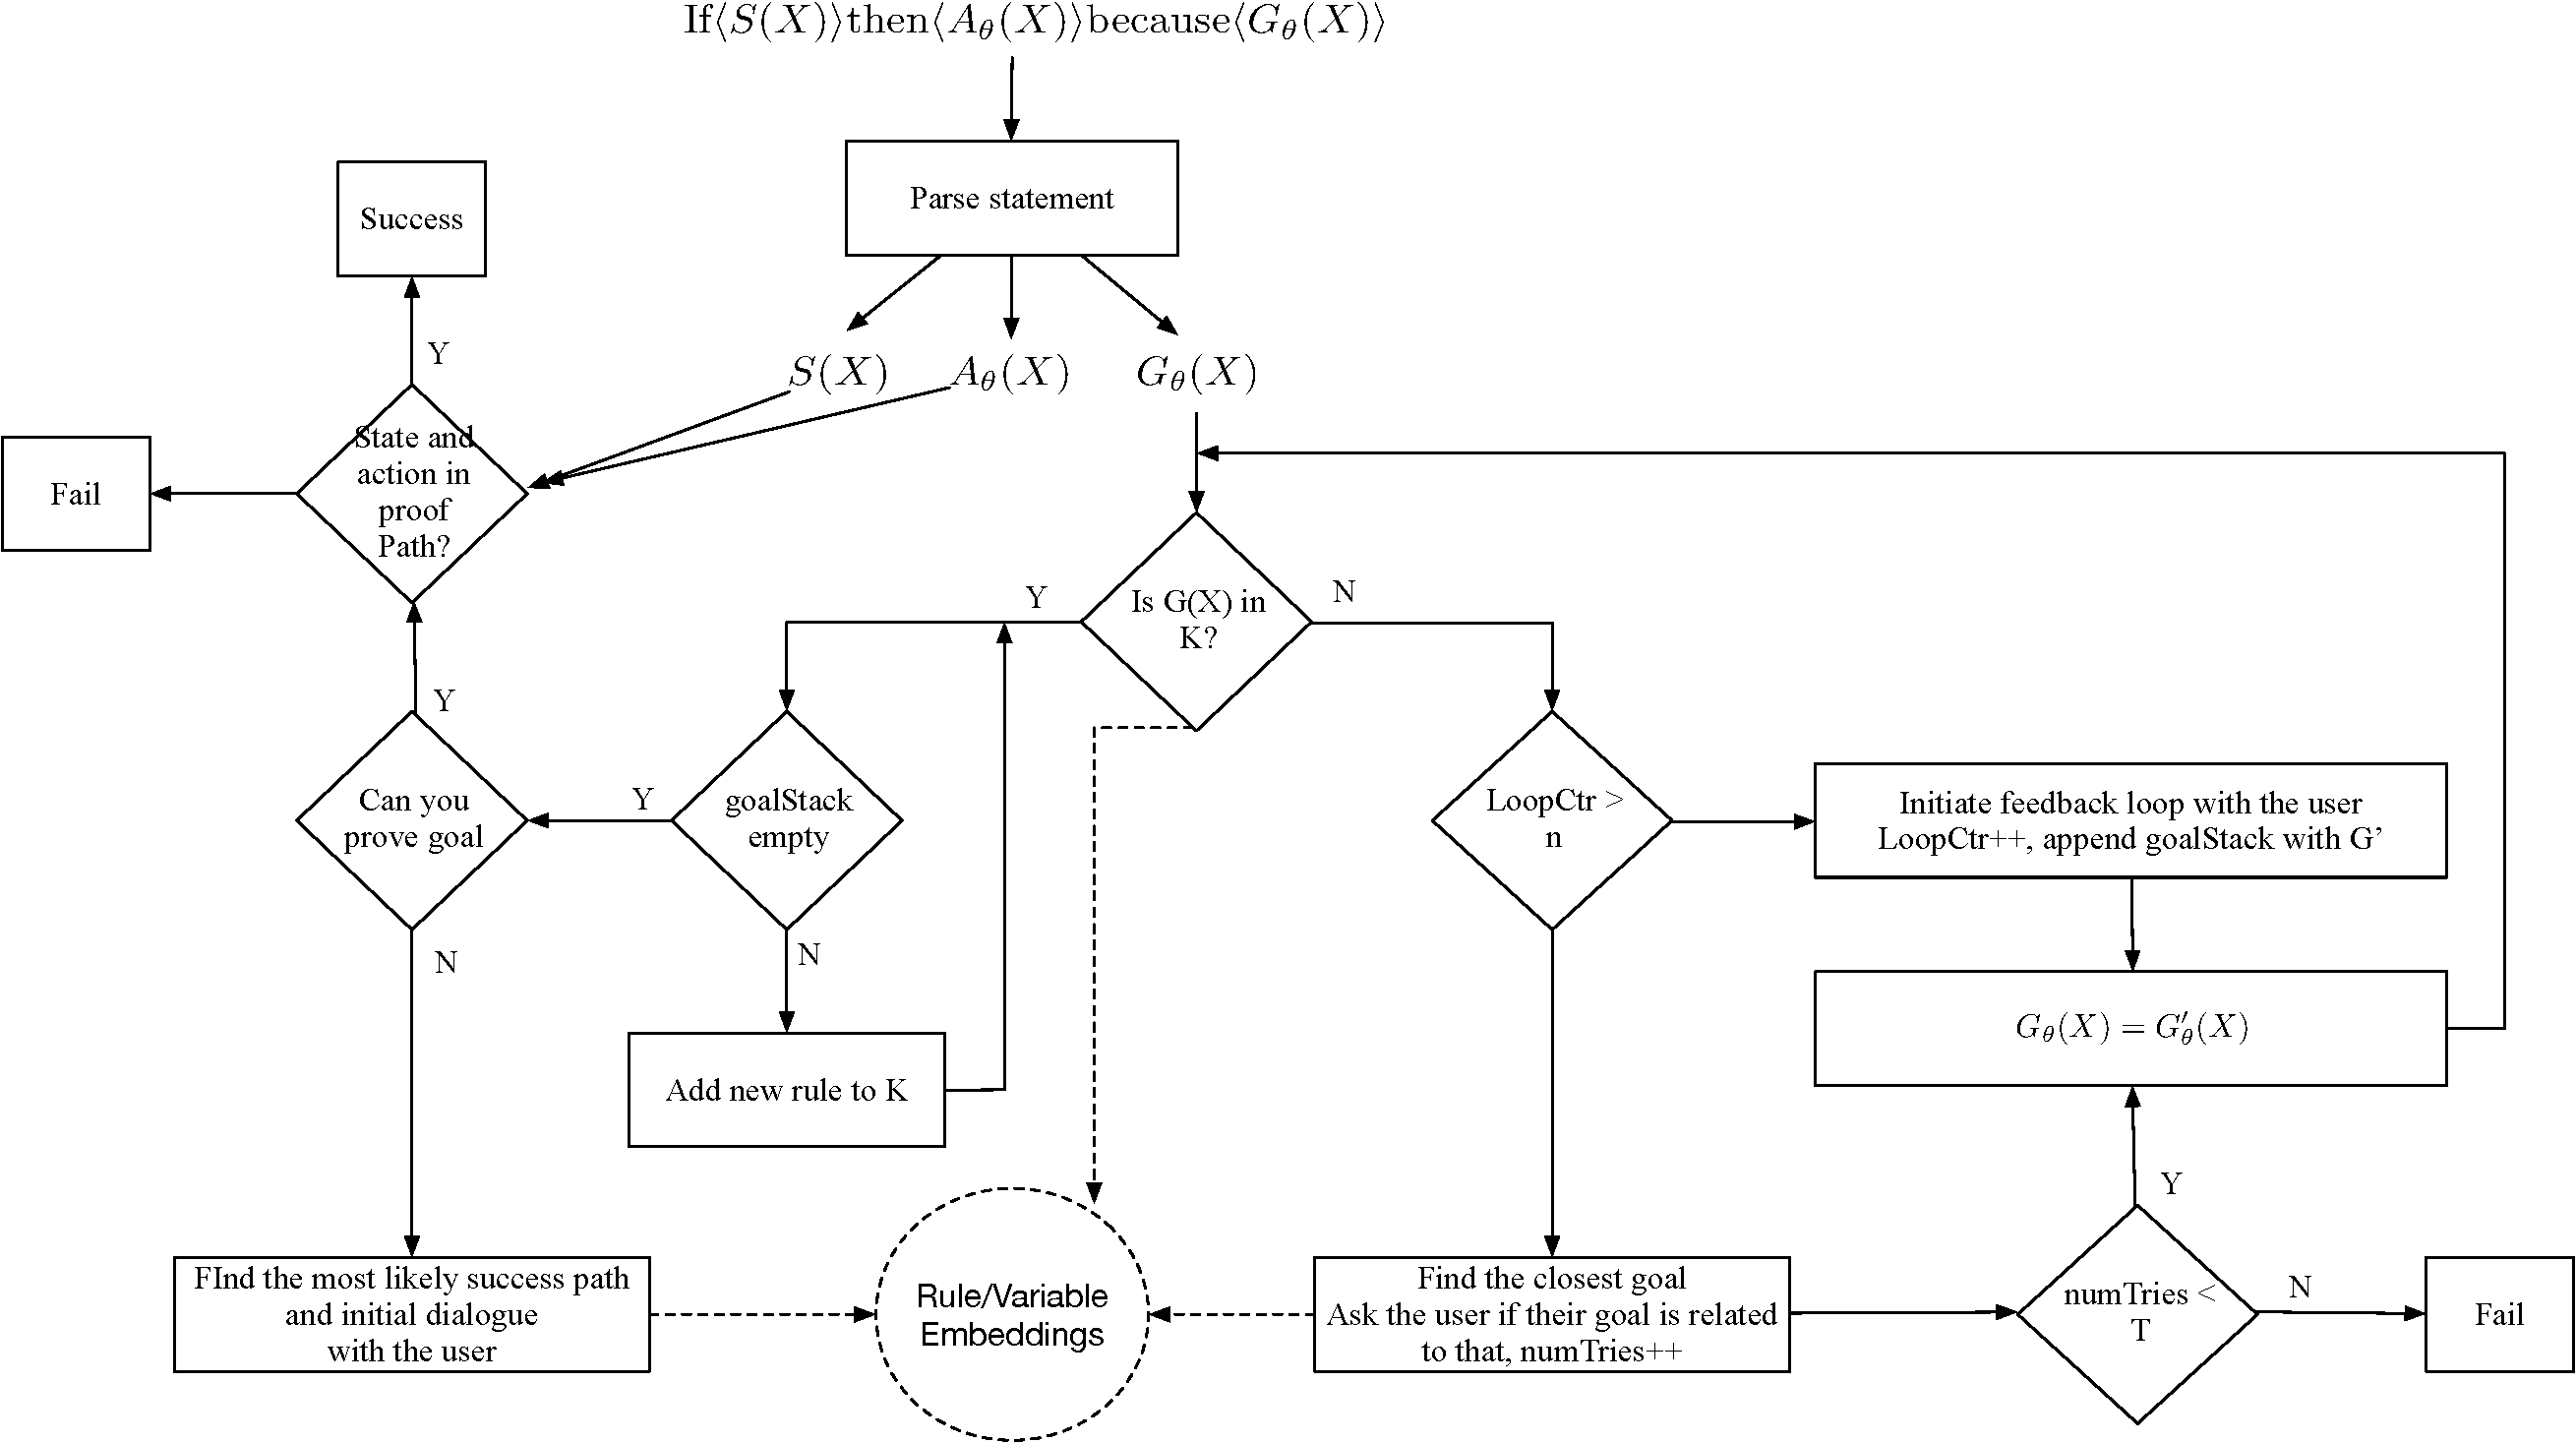
\includegraphics[width=\textwidth]{figs/model.pdf}
    % \caption{Model Architecture \amoscomment{Why 'proposed'? The arrows from S(X) and A(X) make it hard to understand the flow (that is, what happens first, what next). Maybe just remove them or mark it differently (not using arrows).} \facomment{figure is being re-generated}}
    \caption{Model flowchart. $\mathrm{goalStack}$ and the loop variable $i$ are initialized to empty and $0$ respectively. \textcolor{brickred}{Colored text} in the figure represents descriptions.}
    \label{fig:model}
\end{figure}